% ---------------------------------------------------------------------------
%  Mini Transaction Ledger - written explanation
%  MISL Fresher Assessment Project
%
%  Compile with pdfLaTeX. On Overleaf: upload this file, press Recompile.
%  Only standard TeX Live packages are used; nothing needs shell-escape.
% ---------------------------------------------------------------------------

\documentclass[11pt,a4paper]{article}

\usepackage[T1]{fontenc}
\usepackage[utf8]{inputenc}
\usepackage[english]{babel}
\usepackage{lmodern}
\usepackage{microtype}
\usepackage[margin=2.4cm]{geometry}
\usepackage{xcolor}
\usepackage{booktabs}
\usepackage{array}
\usepackage{enumitem}

% Body prose is justified, but a fixed-width table column is not long enough to
% absorb the stretch -- especially here, where cells are full of \texttt{} names
% that TeX will not hyphenate. L{} is a p{} column set ragged right instead.
\newcolumntype{L}[1]{>{\raggedright\arraybackslash}p{#1}}
\usepackage{listings}
\usepackage{caption}
\usepackage{tikz}
\usetikzlibrary{positioning,arrows.meta,fit,backgrounds}
\usepackage[hidelinks]{hyperref}

% --- palette ---------------------------------------------------------------
\definecolor{ink}{HTML}{182B22}
\definecolor{band}{HTML}{EEF3EC}
\definecolor{rule}{HTML}{C6D5CB}
\definecolor{debit}{HTML}{A3231E}
\definecolor{muted}{HTML}{5C6B62}

\lstset{
  basicstyle=\ttfamily\small,
  backgroundcolor=\color{band},
  frame=leftline,
  rulecolor=\color{rule},
  framesep=6pt,
  xleftmargin=10pt,
  breaklines=true,
  columns=fullflexible,
  showstringspaces=false,
  keywordstyle=\color{ink}\bfseries,
  commentstyle=\color{muted}\itshape,
  stringstyle=\color{debit},
}

\captionsetup{font=small,labelfont={bf,color=ink},justification=justified}

% Body text is flush on both margins -- that is the article class default and
% is left in place. What it needs is slack: paragraphs here are dense with
% \texttt{} identifiers, which TeX will not hyphenate, so without extra stretch
% a single long name can push a line past the right margin. `babel` supplies
% English hyphenation patterns and `microtype` tightens the spacing that
% justification produces.
\emergencystretch=1.5em
\hyphenpenalty=200
\tolerance=1200

\title{\vspace{-1.5cm}\textbf{Mini Transaction Ledger}\\[2pt]
       \large Architecture and Internal Workings}
\author{Ekramul Alam}
\date{MISL Fresher Assessment Project \textperiodcentered\ September 2026}

\begin{document}
\maketitle

\section{Overview}

The application is a transaction ledger. Accounts are opened, money is deposited, withdrawn and
transferred between them, and every movement of money is recorded as an immutable ledger entry
that carries the balance it left behind. A transfer is balanced --- one debit and one matching
credit that net to zero. Section~\ref{sec:scope} lists what was deliberately left out.

It is built as three containers started by a single \texttt{docker compose up}: an Angular
frontend served by nginx, a Spring Boot REST backend, and a PostgreSQL database.

The design goal throughout was that the database should never be able to hold a state that is
arithmetically impossible. Balances cannot go negative, an event either lands completely or not at
all, two simultaneous withdrawals cannot both spend the same money, and the stored balance can be
proved to equal the sum of the entries that produced it.

\section{Application architecture}

\subsection{Frontend and backend interaction}

The browser only ever requests paths beginning with \texttt{/api/}. It never knows the backend's
address. In production, nginx serves the compiled Angular files and forwards \texttt{/api/} to the
backend container; in development, the Angular dev server does the same job through
\texttt{proxy.conf.json}.

Because the browser therefore talks to exactly one origin, the browser's same-origin rule is never
triggered, and \textbf{there is no CORS configuration anywhere in this project}. This was a
deliberate architectural choice rather than an omission: a reverse proxy in front of both the
static files and the API removes an entire class of configuration and an entire class of bug.

\begin{figure}[htbp]
\centering
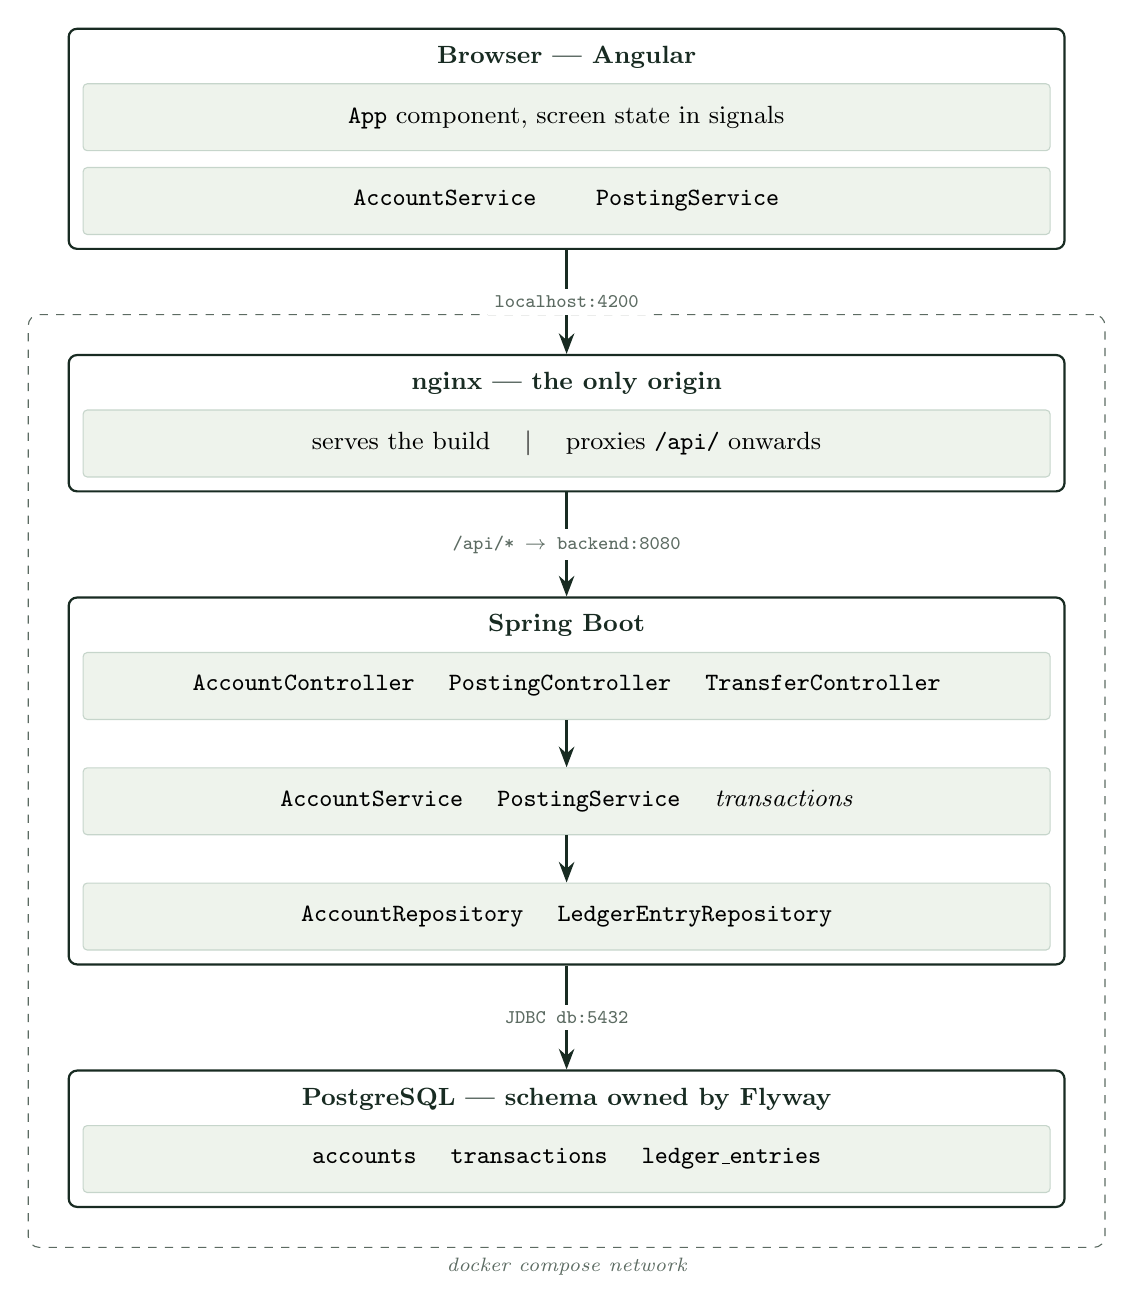
\begin{tikzpicture}[
  % Tier titles live INSIDE their box, so the vertical gaps belong to the
  % arrows alone and nothing can collide with a heading.
  title/.style = {font=\bfseries\small, align=center, inner sep=1pt,
                  text=ink, minimum width=120mm},
  part/.style  = {draw=rule, fill=band, rounded corners=1.5pt, align=center,
                  font=\small, inner sep=4pt, text width=120mm, align=center, minimum height=8.5mm},
  % No fill here. A fit node is drawn after the nodes it surrounds, so a fill
  % would paint over its own contents.
  tier/.style  = {draw=ink, thick, rounded corners=3pt, inner sep=5pt},
  hop/.style   = {-{Stealth[length=2.6mm]}, very thick, draw=ink},
  tag/.style   = {font=\scriptsize\ttfamily, text=muted, fill=white, inner sep=2.5pt},
]

% ----------------------------------------------------------------- browser --
\node[title] (t1) {Browser \textemdash\ Angular};
\node[part, below=1.5mm of t1] (ui) {\texttt{App} component, screen state in signals};
\node[part, below=2mm of ui] (fesvc) {\texttt{AccountService} \qquad \texttt{PostingService}};
\node[tier, fit=(t1)(ui)(fesvc)] (browser) {};

% ------------------------------------------------------------------- nginx --
\node[title, below=17mm of fesvc] (t2) {nginx \textemdash\ the only origin};
\node[part, below=1.5mm of t2] (ngx) {serves the build \quad $\vert$ \quad proxies \texttt{/api/} onwards};
\node[tier, fit=(t2)(ngx)] (web) {};

% -------------------------------------------------------------- spring boot --
\node[title, below=17mm of ngx] (t3) {Spring Boot};
\node[part, below=1.5mm of t3] (ctrl) {\texttt{AccountController} \quad \texttt{PostingController} \quad \texttt{TransferController}};
\node[part, below=6mm of ctrl] (svc) {\texttt{AccountService} \quad \texttt{PostingService} \quad {\itshape transactions}};
\node[part, below=6mm of svc] (repo) {\texttt{AccountRepository} \quad \texttt{LedgerEntryRepository}};
\node[tier, fit=(t3)(ctrl)(svc)(repo)] (boot) {};

% ---------------------------------------------------------------- postgres --
\node[title, below=17mm of repo] (t4) {PostgreSQL \textemdash\ schema owned by Flyway};
\node[part, below=1.5mm of t4] (tables) {\texttt{accounts} \quad \texttt{transactions} \quad \texttt{ledger\_entries}};
\node[tier, fit=(t4)(tables)] (db) {};

% ------------------------------------------------------------------ arrows --
\draw[hop] (browser) -- node[tag]{localhost:4200} (web);
\draw[hop] (web)     -- node[tag]{/api/* $\to$ backend:8080} (boot);
\draw[hop] (boot)    -- node[tag]{JDBC db:5432} (db);
\draw[hop] (ctrl)    -- (svc);
\draw[hop] (svc)     -- (repo);

% --------------------------------------------------- the compose boundary --
\begin{scope}[on background layer]
  \node[draw=muted, dashed, rounded corners=4pt, inner sep=5mm,
        fit=(web)(boot)(db),
        label={[font=\scriptsize\itshape, text=muted]below:docker compose network}] {};
\end{scope}

\end{tikzpicture}
\caption{The whole system. The browser requests only \texttt{/api/} paths and never learns the
backend's address, so every request has one origin and no CORS configuration is needed. Inside the
backend each layer talks only to the one beneath it; repositories are package-private, so no
feature can reach another feature's data without going through its service. Not drawn, because it
sits across all three layers rather than inside one: \texttt{GlobalExceptionHandler}, which turns
any exception that escapes into an \texttt{ApiError} response.}
\label{fig:architecture}
\end{figure}

\subsection{Backend structure}

Figure~\ref{fig:architecture} shows the whole system. The backend is a conventional layered
application, but it is \textbf{packaged by feature rather than by layer}. There is an \texttt{account} package and an \texttt{entry} package, each holding
its own controller, service, repository and entity, instead of a project-wide \texttt{controllers/},
\texttt{services/} and \texttt{repositories/}.

\begin{table}[htbp]
\centering\small
\begin{tabular}{@{}lll@{}}
\toprule
\textbf{Layer} & \textbf{Responsibility} & \textbf{Knows nothing about} \\
\midrule
Controller & bind HTTP, validate, choose the status code & business rules, SQL \\
Service    & business rules, transaction boundaries      & HTTP, JSON \\
Repository & database access                             & why it is being asked \\
\bottomrule
\end{tabular}
\caption{Each layer's responsibility, and what it is deliberately ignorant of.}
\end{table}

Two structural decisions are worth drawing attention to.

\paragraph{Repositories are package-private.} \texttt{AccountRepository} is not declared
\texttt{public}. The posting feature in the \texttt{entry} package therefore \emph{cannot} reach
account data directly --- it has to ask \texttt{AccountService}. The compiler enforces the module
boundary, rather than a naming convention asking politely. A useful consequence is that every
balance change flows through one method, so every balance change is locked; there is no second
path to get wrong.

\paragraph{DTOs at the edge.} Controllers accept and return Java records
(\texttt{CreateAccountRequest}, \texttt{AccountResponse}, \texttt{EntryResponse}), never JPA
entities. The API contract can then evolve independently of the database schema, and no entity is
ever accidentally serialised together with its lazy associations.

\section{Key code components}

\begin{table}[htbp]
\centering\small
\begin{tabular}{@{}L{4.9cm}L{9.6cm}@{}}
\toprule
\textbf{Component} & \textbf{Purpose} \\
\midrule
\texttt{Account} &
Entity holding the balance. Has no setters: the balance changes only through \texttt{credit()} and
\texttt{debit()}, and the overdraft rule lives inside \texttt{debit()} so no caller can forget it. \\
\addlinespace
\texttt{LedgerTransaction} &
One financial event --- a deposit, withdrawal or transfer. Named to avoid being confused with a
database transaction. Carries the client-supplied idempotency key. \\
\addlinespace
\texttt{LedgerEntry} &
One movement of money on one account. Append-only, no setters. Amount is always positive; a
\texttt{direction} of \texttt{DEBIT} or \texttt{CREDIT} carries the sign. \\
\addlinespace
\texttt{AccountService} &
Opens accounts and moves money. Owns the locking, including the ordered lock acquisition that
makes transfers deadlock-free. \\
\addlinespace
\texttt{PostingService} &
Turns a deposit, withdrawal or transfer into one all-or-nothing unit of work: the event row, the
balance change, and the entry rows. \\
\addlinespace
\texttt{GlobalExceptionHandler} &
A single \texttt{@RestControllerAdvice} translating exceptions into HTTP responses, so no service
method ever needs a try-catch. \\
\addlinespace
\texttt{ApiError} &
One error shape for the whole API, so a client never has to guess what a failure looks like. \\
\addlinespace
Flyway migrations &
\texttt{V1} creates \texttt{accounts}; \texttt{V2} creates \texttt{transactions} and
\texttt{ledger\_entries} with their constraints and indexes. \\
\bottomrule
\end{tabular}
\caption{The components that carry the design.}
\end{table}

On the frontend there is one page and therefore one component. Two services,
\texttt{AccountService} and \texttt{PostingService}, own every HTTP call; the component holds the
screen state in Angular signals and exposes one method per endpoint. There is no router, no state
management library and no component library --- for a single screen each of those would be
ceremony rather than structure.

\section{How the API works internally}

The clearest way to show the internals is to follow one request the whole way down. Taking
\texttt{POST /api/transfers}, with the transactional part of it drawn in
Figure~\ref{fig:transaction}:

\begin{enumerate}[leftmargin=*, itemsep=3pt]
  \item \textbf{nginx} matches the \texttt{/api/} prefix and proxies to \texttt{backend:8080},
        resolving the container by its Compose service name over Docker's internal DNS.
  \item \textbf{\texttt{DispatcherServlet}}, Spring's front controller, matches the URL and HTTP
        method to \texttt{TransferController.transfer(...)}.
  \item \textbf{Jackson} deserialises the request body into a \texttt{TransferRequest} record.
  \item \textbf{\texttt{@Valid}} runs Bean Validation \emph{before} the method body executes. If a
        constraint fails, a \texttt{MethodArgumentNotValidException} is thrown and the advice
        returns \texttt{400} listing every rejected field --- not merely the first.
  \item \textbf{\texttt{PostingService.transfer}} is annotated \texttt{@Transactional}. Everything
        from this point is one unit of work. It writes the \texttt{transactions} row, then asks
        \texttt{AccountService} to move the money.
  \item \textbf{\texttt{AccountService.moveMoney}} locks both accounts with
        \texttt{SELECT \ldots\ FOR NO KEY UPDATE}, \textbf{always taking the lower account id
        first}, checks that the currencies match, and applies the debit and the credit.
  \item Two \texttt{ledger\_entries} rows are written, each recording the balance it left behind.
  \item \textbf{Commit.} Hibernate flushes both balance updates and both entries together.
  \item The controller returns \texttt{201 Created} with the debit entry and the credit entry.
\end{enumerate}

\begin{figure}[htbp]
\centering
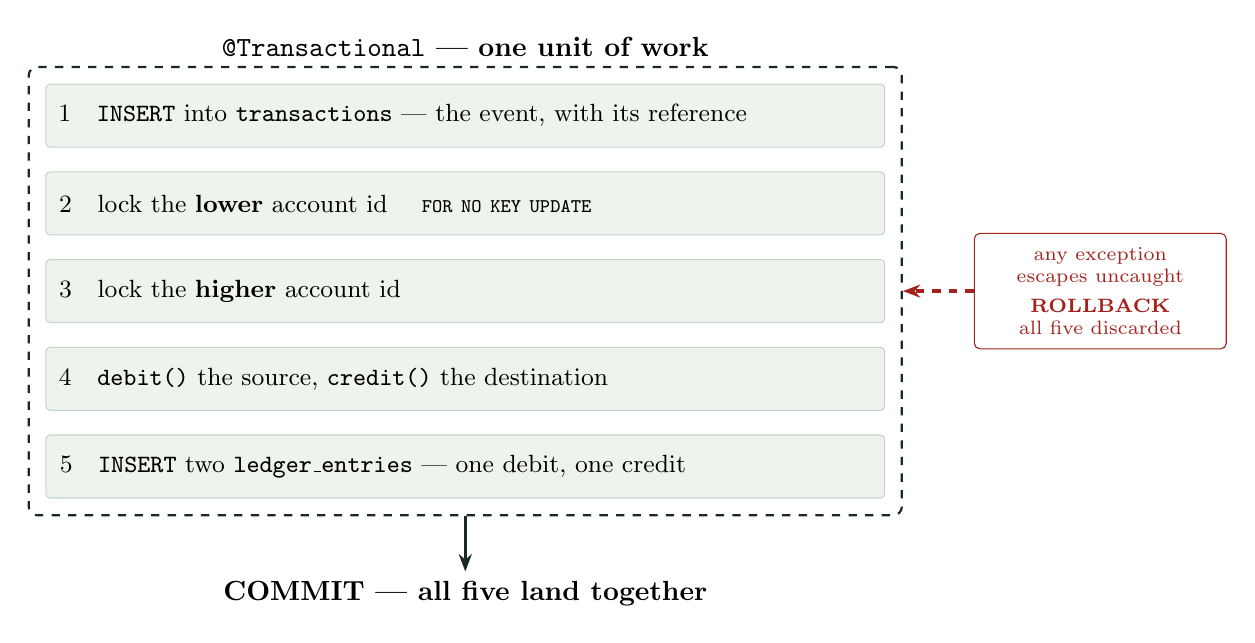
\begin{tikzpicture}[
  node distance=3mm,
  txstep/.style  = {draw=rule, fill=band, rounded corners=1.5pt, align=left,
                  font=\small, inner sep=5pt, text width=103mm, minimum height=8mm},
  flow/.style  = {-{Stealth[length=2.2mm]}, very thick, draw=ink},
  undo/.style  = {-{Stealth[length=2.2mm]}, very thick, draw=debit, dashed},
]

\node[txstep] (s1) {1\quad \texttt{INSERT} into \texttt{transactions} --- the event, with its reference};
\node[txstep, below=of s1] (s2) {2\quad lock the \textbf{lower} account id \quad {\scriptsize\ttfamily FOR NO KEY UPDATE}};
\node[txstep, below=of s2] (s3) {3\quad lock the \textbf{higher} account id};
\node[txstep, below=of s3] (s4) {4\quad \texttt{debit()} the source, \texttt{credit()} the destination};
\node[txstep, below=of s4] (s5) {5\quad \texttt{INSERT} two \texttt{ledger\_entries} --- one debit, one credit};

\node[draw=ink, thick, dashed, rounded corners=3pt, inner sep=6pt, fit=(s1)(s2)(s3)(s4)(s5),
      label={[font=\bfseries]above:\texttt{@Transactional} --- one unit of work}] (tx) {};

\node[below=7mm of tx, font=\bfseries] (commit) {COMMIT --- all five land together};
\draw[flow] (tx.south) -- (commit.north);

\node[draw=debit, fill=white, rounded corners=2pt, align=center, font=\scriptsize,
      text=debit, inner sep=5pt, right=9mm of tx, minimum width=32mm] (rb)
  {any exception\\ escapes uncaught\\[3pt]\textbf{ROLLBACK}\\ all five discarded};
\draw[undo] (rb.west) -- (tx.east);

\end{tikzpicture}
\caption{A transfer, from the service's point of view. Because nothing catches the exception, a
failure at step~4 --- insufficient balance, say --- also throws away the event row written at
step~1. The ledger never keeps a record of something that did not happen.}
\label{fig:transaction}
\end{figure}

\subsection{Why there is no try-catch in the service layer}

If any step above throws, the exception is allowed to escape. Nothing catches it. Spring sees an
unchecked exception leave a \texttt{@Transactional} method and rolls the whole transaction back ---
so the \texttt{transactions} row written in step~5 is discarded along with everything else.

This is the reason the service layer contains no defensive try-catch. Catching an exception inside
a transactional method would let Spring see a clean return and \textbf{commit a half-finished
operation}. The ledger would then hold a record of an event that never actually happened. Errors
are instead translated once, at the boundary, by \texttt{GlobalExceptionHandler}.

That handler deliberately does \emph{not} declare an \texttt{@ExceptionHandler(Exception.class)}.
A catch-all in a \texttt{@RestControllerAdvice} is resolved before Spring's own exception
resolvers, so it would intercept the framework's exceptions too --- turning malformed JSON, an
unknown path and a wrong HTTP method into \texttt{500}s instead of the \texttt{400},
\texttt{404} and \texttt{405} they should be.

The cost of that choice is that those framework errors keep Spring Boot's default error body,
which has no \texttt{message} field. Producing one shape \emph{and} correct framework statuses
means extending \texttt{ResponseEntityExceptionHandler} and overriding each framework exception
in turn.

\subsection{Duplicate protection}

Every posting request carries a \texttt{reference}, a UUID generated by the client and stored under
a unique constraint on \texttt{transactions}. If a client retries a request whose response was
lost, the second insert violates that constraint and the money moves exactly once.

This is a duplicate \emph{guard} rather than full idempotent replay: the retry is answered with
\texttt{409}, not with the original response.

\begin{lstlisting}
POST /api/accounts/7/deposits
{ "reference": "b4f1...c2", "amount": "1500.75", "description": "salary" }
\end{lstlisting}

\subsection{Money and precision}

Amounts are \texttt{NUMERIC(19,4)} in PostgreSQL and \texttt{BigDecimal} in Java, never
\texttt{double}. Binary floating point cannot represent 0.1 exactly, and a rounding error invisible
in a user interface is unacceptable in a ledger.

Comparisons use \texttt{compareTo} rather than \texttt{equals}, because two \texttt{BigDecimal}
values of the same amount but different scale --- \texttt{10.5} and \texttt{10.5000} --- are not
\texttt{equals} to each other, though they do compare as equal.

The frontend receives balances as JSON numbers and only ever displays them. No arithmetic on money
happens in the browser, where the only available numeric type is a floating-point double.

\section{Correctness under concurrency}

This is where most of the engineering went, so it is worth stating explicitly.

\paragraph{Lost updates.} Account rows are read with
\texttt{@Lock(LockModeType.PESSIMISTIC\_WRITE)}. On PostgreSQL, Hibernate renders this as
\texttt{SELECT \ldots\ FOR NO KEY UPDATE}, which blocks any other transaction attempting to write
the same row. Without it, two simultaneous withdrawals both read the old balance, both decide there
is enough money, and both succeed.

\paragraph{Deadlock.} A transfer locks two rows, so ordering matters. If $A \rightarrow B$ locked
$A$ then $B$ while $B \rightarrow A$ locked $B$ then $A$, each would hold what the other needs and
neither could finish. \texttt{moveMoney} therefore always locks the \textbf{lower account id
first}, whichever direction the money is going, so both transfers queue for the same row: one waits
and the other proceeds.

\paragraph{The stored balance.} \texttt{accounts.balance} is a materialized derived aggregate. The
entries are canonical; the column exists only so that reading a balance does not require scanning
an account's whole history. Three safeguards keep it honest: only \texttt{credit()} and
\texttt{debit()} write it, it is written in the same transaction as the entry that causes it, and a
test replays the entries and asserts they sum to it.

\paragraph{Evidence.} Both concurrency tests were run once with their safeguard deliberately
removed, to confirm that they can actually fail:

\begin{table}[htbp]
\centering\small
\begin{tabular}{@{}L{4.4cm}L{3.4cm}L{6.4cm}@{}}
\toprule
\textbf{Test} & \textbf{Safeguard removed} & \textbf{Result} \\
\midrule
Ten simultaneous withdrawals of the full balance &
\texttt{PESSIMISTIC\_WRITE} &
All ten succeeded. 1000 withdrawn against a balance of 100, and the balance still read zero. \\
\addlinespace
Ten transfers, five in each direction &
lowest-id-first ordering &
Nine of ten died with SQLSTATE \texttt{40P01}, \emph{deadlock detected}. \\
\bottomrule
\end{tabular}
\caption{Control experiments. A passing test proves nothing until it has been seen to fail.}
\end{table}

Neither concurrency test is annotated \texttt{@Transactional}. A test transaction would hold the
very rows the worker threads are competing for, and the test would hang rather than fail;
concurrency can only be observed against committed data.

\section{Docker setup}

\texttt{docker-compose.yml} defines three services.

\begin{table}[htbp]
\centering\small
\begin{tabular}{@{}llL{8.4cm}@{}}
\toprule
\textbf{Service} & \textbf{Base image} & \textbf{Notes} \\
\midrule
\texttt{db}       & \texttt{postgres:16}  & Named volume, so data survives \texttt{docker compose down} and container rebuilds. Host port 5433 avoids clashing with a locally installed PostgreSQL. \\
\addlinespace
\texttt{backend}  & built multi-stage     & Waits for the database to be \emph{healthy}, not merely started. \\
\addlinespace
\texttt{frontend} & built multi-stage     & nginx serving the compiled application and proxying \texttt{/api} to the backend. \\
\bottomrule
\end{tabular}
\caption{The three services and why each is configured as it is.}
\end{table}

\paragraph{Multi-stage builds.} The backend compiles in a full JDK image and runs in a JRE image,
so no compiler, no Maven and no source code reach the runtime image; it also runs as a non-root
user, so a compromised application cannot own its container. The frontend builds with Node and runs
on nginx, so neither Node nor \texttt{node\_modules} ship.

\paragraph{Layer caching.} In both Dockerfiles the dependency manifest is copied and resolved
\emph{before} the source is copied. Docker caches each step, so dependencies are re-downloaded only
when \texttt{pom.xml} or \texttt{package-lock.json} changes, not on every code edit.

\paragraph{Healthchecks.} ``The container is running'' is not the same statement as ``PostgreSQL is
ready to accept queries''. The database declares a \texttt{pg\_isready} healthcheck, and the
backend depends on \texttt{service\_healthy}, so it never starts against a database that is still
initialising.

\paragraph{Configuration.} Connection details come from environment variables with local defaults,
so a reviewer can start the project without creating any files. Nothing is hard-coded, and a real
deployment overrides them with a \texttt{.env} file.

\paragraph{Single-page routing.} nginx serves \texttt{try\_files \$uri \$uri/ /index.html}, so
refreshing the browser on any path returns the application rather than a 404.

\section{Testing}

\begin{itemize}[leftmargin=*, itemsep=2pt]
  \item \textbf{Context test} --- starting Spring proves every bean wires and, because
        \texttt{ddl-auto=validate}, that the entities still match the migrated schema.
  \item \textbf{Concurrent withdrawal} --- ten threads, one balance, exactly one winner, and the
        nine rolled-back attempts leave no \texttt{transactions} rows behind.
  \item \textbf{Concurrent transfer} --- ten transfers in both directions at once; none deadlock
        and the money is conserved.
  \item \textbf{Reconciliation} --- replaying an account's entries reproduces its stored balance.
  \item \textbf{Frontend} --- the component renders, and the UUID fallback used outside a secure
        browsing context produces valid v4 references.
\end{itemize}

\section{Scope}\label{sec:scope}

Deliberately out of scope for this assessment, each a decision rather than an oversight:

\begin{itemize}[leftmargin=*, itemsep=2pt]
  \item \textbf{Authentication and authorization} --- the brief places JWT under Problem~2.
        Production would need an owner on each account, an ownership check on the debit side of a
        transfer, and an actor recorded on every transaction.
  \item \textbf{Full double-entry} --- a transfer is balanced, but a deposit has a single leg. A
        general ledger gives it a settlement counterparty, which makes \emph{every entry, signed by
        direction, sums to zero} a testable invariant.
  \item \textbf{Pagination, lock timeouts, a currency reference table, and CI.}
\end{itemize}

\vspace{4mm}
\noindent\textcolor{muted}{\rule{\linewidth}{0.4pt}}
\vspace{1mm}

\noindent\small The full source, including the README with setup instructions, is in the
accompanying repository.

\end{document}
